
% \subsection*{subsection name}
%
% we choose $\q(\nuk \vert \eta)$ to be logit-normally distributed,
% and express the expectations in \eqref{stick_expectations} as Gaussian integrals.
% Define
% \begin{align*}
%   \tilde \nuk := \log\left(\frac{\nuk}{1 - \nuk}\right),
% \end{align*}
% which will be normally distributed under our choice of a
% logit-normal $\q(\nuk \vert \eta)$.
%
% Let $\lnumean_\k$ and $\lnusd_\k$ be entries of $\eta$ corresponding to
% the logit-normal parameters of $\nuk$.
%
%
% In order to optimize the variational objective \eqref{vb_optimization} we see
% from \eqref{stick_log_post} that we need to evaluate or approximate expectations
% of the form
% %
% \begin{align*}
% %
% \expect{\q(\nuk \vert \eta)}{\log \nuk}
% \textrm{,}\quad
% \expect{\q(\nuk \vert \eta)}{\log (1 - \nuk)}
% \textrm{,}\quad\textrm{and}\quad
% \expect{\q(\nuk \vert \eta)}{\log \pstick(\nuk)}.
% %
% \end{align*}
%
%
%
%
% First, define a version of $\nuk$ that is not constrained to $(0,1)$:
% %
% \begin{align}\eqlabel{lnuk_transform}
% %
% \lnuk :={} \log \left( \frac{\nuk}{1 - \nuk} \right)
% \quad\Leftrightarrow\quad
% \nuk :={} \frac{\exp(\lnuk)}{1 + \exp(\lnuk)}.
% %
% \end{align}
% %
It will be useful later to have at hand the transform between densities
expressed in the space of $\nu$ and $\lnu$, which is given by
%
\begin{align}\eqlabel{lnuk_derivatives}
%
\fracat{d \lnu_\k}{ d\nuk}{\nuk} ={}
%     \frac{1-\nuk}{\nuk}
%     \left(\frac{1}{1 - \nuk} + \frac{\nuk}{(1 - \nuk)^2} \right)
% \\={}& \frac{1}{\nuk} + \frac{1}{1 - \nuk}
% \\={}&
    \frac{1}{\nuk (1 - \nuk)} \mathand
%
\fracat{d \nuk}{ d\lnuk}{\lnuk} ={}
    \frac{\exp(\lnuk)}{(1 + \exp(\lnuk))^2}.
%
\end{align}
% %
% We wish to let $\lnu_\k$ be distributed normally under the variational
% distribution.  Let $\lnumean_\k$ and $\lnusd_\k$ be entries of the parameter
% vector $\eta$, and write
% %
% \begin{align}\eqlabel{lnuk_vb_approximation}
% %
% \q(\lnu_\k \vert \eta) ={}& \normdist{\lnu_\k \vert \lnumean_\k, \lnusd_\k}
% \Rightarrow \\
% \q(\nuk \vert \eta) ={}&
%     \normdist{\log \left( \frac{\nuk}{1 - \nuk} \right)
%         \vert \lnumean_\k, \lnusd_\k}
%     \left|\fracat{d \lnu_\k}{ d\nuk}{\nuk}\right|
% \nonumber\\={}&
% \normdist{\log \left( \frac{\nuk}{1 - \nuk} \right)
%         \vert \lnumean_\k, \lnusd_\k}
%     \left|\frac{1}{\nuk (1 - \nuk)}\right|.
% \nonumber
% %
% \end{align}
% %
% Given this, we can approximate expectations of smooth functions
% $f(\nuk)$ using GH quadrature with $\ngh$ knots,
% located at $\xi_g$, weighted by $\omega_g$:
% %
% \begin{align}\eqlabel{gh_integral}
% %
% \expect{\q(\nuk \vert \eta)}{f(\nuk)} ={}&
% \expect{\q(\lnu_\k \vert \eta)}
%        {f\left(\frac{\exp(\lnu_\k)}{1 + \exp(\lnu_\k)}\right)}
% \nonumber\\\approx{}&
%     \sum_{g=1}^{\ngh} \omega_g f\left(\lnusd_\k \xi_{g} + \lnumean_\k\right)
%  \nonumber\\=:{}&
% \expecthat{\q(\nuk \vert \eta)}{f(\nuk)}.
% %
% \end{align}
% %
% Conveniently, $\expecthat{\q(\nuk \vert \eta)}{f(\nuk)}$ is a differentiable
% function of $\lnumean_\k$ and $\lnusd_\k$, and so also of $\eta$.  (This
% technique is similar to the ``reparameterization trick,'' only using
% GH points rather than standard normal draws.)

\hrulefill

In the regression example (MICE BNP PROCESS), $\zeta$ includes
the additive shifts, $\zeta := (\beta, \z, \nu, \b)$.

The variational approximation for the topic model
(STRUCTURE BNP PROCESS) is similarly mean-field: the distribution on
stick-breaking proportions $\nu$ factorizes over both individuals $\n$ and
components $\k$, while the assignments $\z$ factorize over individuals $\n$,
loci $\l$, and chromosomes $\i$. For the regression model
(MICE BNP PROCESS), all terms in the variational approximation
fully-factorize except for the cluster assignments $\z$ and additive shifts
$\b$. While we assume $(\z, \b)$ to be independent from all other latent
variables under $\q$, we will allow conditional dependence between $\z$ and $\b$
(\appref{app_mice}).




\hrulefill


% This is necessary here becuase it is a condition under which we have
% differentiability.  Alternatively, we could define it later when
% stating our differentiability theorem...
The KL divergence of \eqref{kl_def} contains a term of the form $\expect{\q(\nuk
\vert \eta)}{\log \pstick(\nuk)}$.  Since we will be considering generic
densities $\pstick(\nuk)$, we will need to compute this integral numerically.
To facilitate numerical integration, we model the sticks using a logit-normal
distribution as follows.  Define
%
\begin{align*}
%
\lnuk := \log\left(\frac{\nuk}{1 - \nuk}\right),
%
\end{align*}
%
and choose $\q(\lnu_\k \vert \eta)$ to be normally distributed.  This then
induces a logit-normal distribution on our original variable of interest,
$\nuk$.  See STICK EXPECTATIONS below for more details.




\hrulefill




%%%%%%%%%%%%%%%%%%%%%%%%%%%%%%%%%%%%%%%%%%%%%%%%%%%%%%%%%%%%%%%%%%%%%%%%%%%%
%
% We conclude this section with a brief remark about computing the expectation
% $\crosshessian$ in our BNP sensitivity analysis.
% We are interested in sensitivity to the stick-breaking distribution,
% so only the prior terms on stick-breaking proportions
% $\nu = (\nu_1, ..., \nu_{\kmax - 1})$ depends on $t$.
% Because the elements of $\nu$ fully factorize
% under both the prior and the variational distributions,
% $\crosshessian$ decomposes as
% \begin{align}
%   \crosshessian &=
%   \sum_{\k=1}^{\kmax - 1}
%           \expect{\q(\nuk \vert \eta)}
%                  {
%                  \lqgrad{\nuk \vert \etaopt}
%                  \fracat{\log \pstick(\nuk \vert \t)}{\partial \t}{\t = 0}
%                  } \notag\\
%   &= \sum_{\k=1}^{\kmax - 1}
%          \evalat{\nabla_\eta \expect{\q(\nuk \vert \eta)}
%                 {
%                 \fracat{\log \pstick(\nuk \vert \t)}{\partial \t}{\t = 0}
%                 }}{\eta = \etaopt(0)},
% \eqlabel{sens_mixed_partial}
% \end{align}
% where we assumed that $\q(\theta \vert \eta)$ is normalized, so
% $\lqgradbar{\theta \vert \etaopt} = \lqgrad{\theta \vert \etaopt}$,
% and that the assumptions of \thmref{etat_deriv} hold, so we
% can freely exchange derivatives with expectations.
%
% We approximate the expectation using GH quadrature (\eqref{gh_integral}), with
% $f(\nu_k) = \fracat{\log \pstick(\nuk \vert \t)}{\partial \t}{\t = 0}$. In all
% the functional forms for $\t \mapsto \pstick(\nuk \vert \t)$ considered below,
% $f(\nu_k)$ can be provided in either closed-form or computed with automatic
% differentiation. The resulting GH approximation is a deterministic function of
% $\eta$, and thus the gradient in \eqref{sens_mixed_partial} can be computed with
% another application of automatic differentiation. Note that $\crosshessian$ is
% sparse in \eqref{sens_mixed_partial}: it is zero for all entries of $\eta$ other
% than those that parameterize the sticks.
%

\hrulefill

% \section{Differentiability}\seclabel{differentiability}
% Although \corref{etafun_deriv_form} is explicitly about a fixed $\phi$,
it suggests an intriguing result if it is taken to hold for all $\phi$ in some
ball, $\ball_p(\delta) := \{\phi: \norm{\phi}_{\lambda,p} \le \delta \}$.
Specifically, let $q^{-1} + p^{-1} = 1$ and observe that, by Holder's inequality,
%
\begin{align*}
%
\sup_{\phi \in \ball_p(\delta)} \fracat{d \etaopt(\t \phi)}{d \t}{0} ={}&
    \sup_{\phi \in \ball_p(\delta)}
        \int \infl_p(\theta) \phi(\theta) \lambda(d\theta)
\\\le{}&
    \sup_{\phi \in \ball_p(\delta)}
        \left( \int \abs{\infl_p(\theta)}^{1/q} \lambda(d\theta) \right)^q
        \left( \int \abs{\phi(\theta)}^{1/p} \lambda(d\theta)\right)^p
\\={}&
\delta \left( \int \abs{\infl_p(\theta)}^{1/q} \lambda(d\theta) \right)^q,
%
\end{align*}
%
with equality at the ``worst-case'' perturbation
%
\begin{align*}
%
\phi^*(\theta) \propto \abs{\infl_p(\theta)}^{p/q}.
%
\end{align*}
%
The constant of proportionality in the preceding display must be adjusted so
that $\norm{\phi^*(\theta)}_{\lambda,p} = \delta$.  These ``worst-case''
perturbations are the variational Bayes analogues of the corresponding
``worst-case'' for exact Bayesian posteriors in \citet{gustafson:1996:local}.

The worst-case perturbation can be difficult to interpret for several reasons.
First of all, although the ``size'' of a perturbation in $\lp{\lambda,p}$ has
many attractive theoretical properties, it can be hard to have a subjective
opinion about.  Note that the predicted effect of the perturbation is linear in
the $\delta$ in $\ball_p(\delta)$ over which you are taking a supremum; to a
large extent, whether or not a problem is ``robust'' under the perturbation
$\phi^*(\theta)$ will depend on how large $\delta$ is allowed to be, and it can
be difficult to have a strong {\em a priori} opinion about how large $\delta$
should be.  Additionally, the form of $\phi^*(\theta)$ can appear unreasonably
adversarial. Note that the influence function $\psi(\theta)$ is proportional to
the variational posterior $\q(\theta \vert \etaopt)$.  As a result,
$\phi^*(\theta)$ will tend to add and remove a great deal of prior mass
immediately in the vicinity of the posterior mass.  For these reasons,
one might wish to use the influence function more as an informal guide to
selecting and testing perturbations that are likely to be influential.

Whether formally or informally, however, when using a linear approximation to
searching over a in infinite dimensional space, one needs to be concerned about
at least two fundamental properties of your derivative.  First, one must ask
whether the derivative even exists for every $\phi \in \ball_p(\delta)$. More
stringenty, one should also ask whether the derivative forms a uniformly good
approximation to the original function for every $\phi \in \ball_p(\delta)$.
These two properties are formalized in functional analysis by the following
definition.

%%%%%%%%%%%%%%%%%%%%%%%%%%%%%%%%%%%%%%%%%%%%%%%%%%%%%%%%%%%%%%%%%%%%%%%%%%%
%%%%%%%%%%%%%%%%%%%%%%%%%%%%%%%%%%%%%%%%%%%%%%%%%%%%%%%%%%%%%%%%%%%%%%%%%%%
\begin{defn}\deflabel{diffable_classes}
    (\citep[Definition 4.5]{zeidler:2013:functional})
%
Let $B_1$ and $B_2$ denote Banach spaces, and let $\ball_1 \subseteq B_1$ define
an open neighborhood of $\phi_0 \in B_1$.  Fix a function $f: \ball_1
\mapsto B_2$.

The function $f$ is {\em directionally differentiable} (also known as a Gateaux
differentiable) if there exists a bounded linear functional $f^{\mathrm{lin}}:
B_1 \mapsto B_2$ such that the following condition holds for any
$\phi$ with $\norm{\phi - \phi_0} < \infty$:
%
\begin{align*}
%
%\textrm{For any }\phi\textrm{ with }\norm{\phi - \phi_0} < \infty\textrm{, }
\lim_{t \rightarrow 0}
    \frac{f(\phi) - f(\phi_0) -
          f^{\mathrm{lin}}(t (\phi - \phi_0) )
         }{t} \rightarrow 0.
%
\end{align*}
%

Similarly, the function $f$ is {\em boundedly differentiable} (also known as
Fr{\'echet} differentiable) at $\phi_0$ if we can take the limit uniformly in
$\phi$:
%
\begin{align*}
%
\lim_{t \rightarrow 0}
    \sup_{\phi: \norm{\phi - \phi_0} = 1}
    \frac{f(\phi) - f(\phi_0) -
          f^{\mathrm{lin}}(t (\phi - \phi_0))
         }{t} \rightarrow 0.
%
\end{align*}
%
\end{defn}
%%%%%%%%%%%%%%%%%%%%%%%%%%%%%%%%%%%%%%%%%%%%%%%%%%%%%%%%%%%%%%%%%%%%%%%%%%%

Note that we used the same notation $f^{\mathrm{lin}}$ for both derivatives in
\defref{diffable_classes}.  In fact, if a function is Fr{\'e}chet differentiable
then the two derivatives must coincide \citep[Proposition
4.8]{zeidler:2013:functional}, which justifies our presumptuous notation.

In order to motivate our concern, let us consider the following simple example.
It is possible for functions to be directionally but not boundedly
differentiable even in $\mathbb{R}^2$, as the following example demonstrates.

%%%%%%%%%%%%%%%%%%%%%%%%%%%%%%%%%%%%%%%%%%%%%%%%%%%%%%%%%%%%%%%%%%%%%%%%%
%%%%%%%%%%%%%%%%%%%%%%%%%%%%%%%%%%%%%%%%%%%%%%%%%%%%%%%%%%%%%%%%%%%%%%%%%
\begin{ex}\exlabel{r2_pathological}
%
Consider $(x_1, x_2) \in \mathbb{R}^2$ and the polar coordinates $r :=
\sqrt{x_1^2 + x_2^2}$ and $\theta := \arctan(x_2 / x_1)$.  Let $\{\pi k: k \in
\mathbb{Z} \}$ denote integer multiples of $\pi$.  Define
%
\begin{align*}
%
f(r, \theta) := \begin{cases}
    \left(\frac{r}{| \sin \theta |}\right)^2
        & \textrm{when } \theta \notin \{\pi k: k \in \mathbb{Z}\}
        \textrm{ and } r > 0 \\
    0. & \textrm{when } \theta \in \{\pi k: k \in \mathbb{Z}
        \} \textrm{ or }r = 0
%
\end{cases}
%
\end{align*}
%
%%%%%%%%%%%%%%%%%%%%%%%%%%%%%%%%%%%%%%%%%%%%%%%%%%%%%%%%%%%%%%%%%%%%%%%%%
%%%%%%%%%%%%%%%%%%%%%%%%%%%%%%%%%%%%%%%%%%%%%%%%%%%%%%%%%%%%%%%%%%%%%%%%%
\begin{figure}[h!]

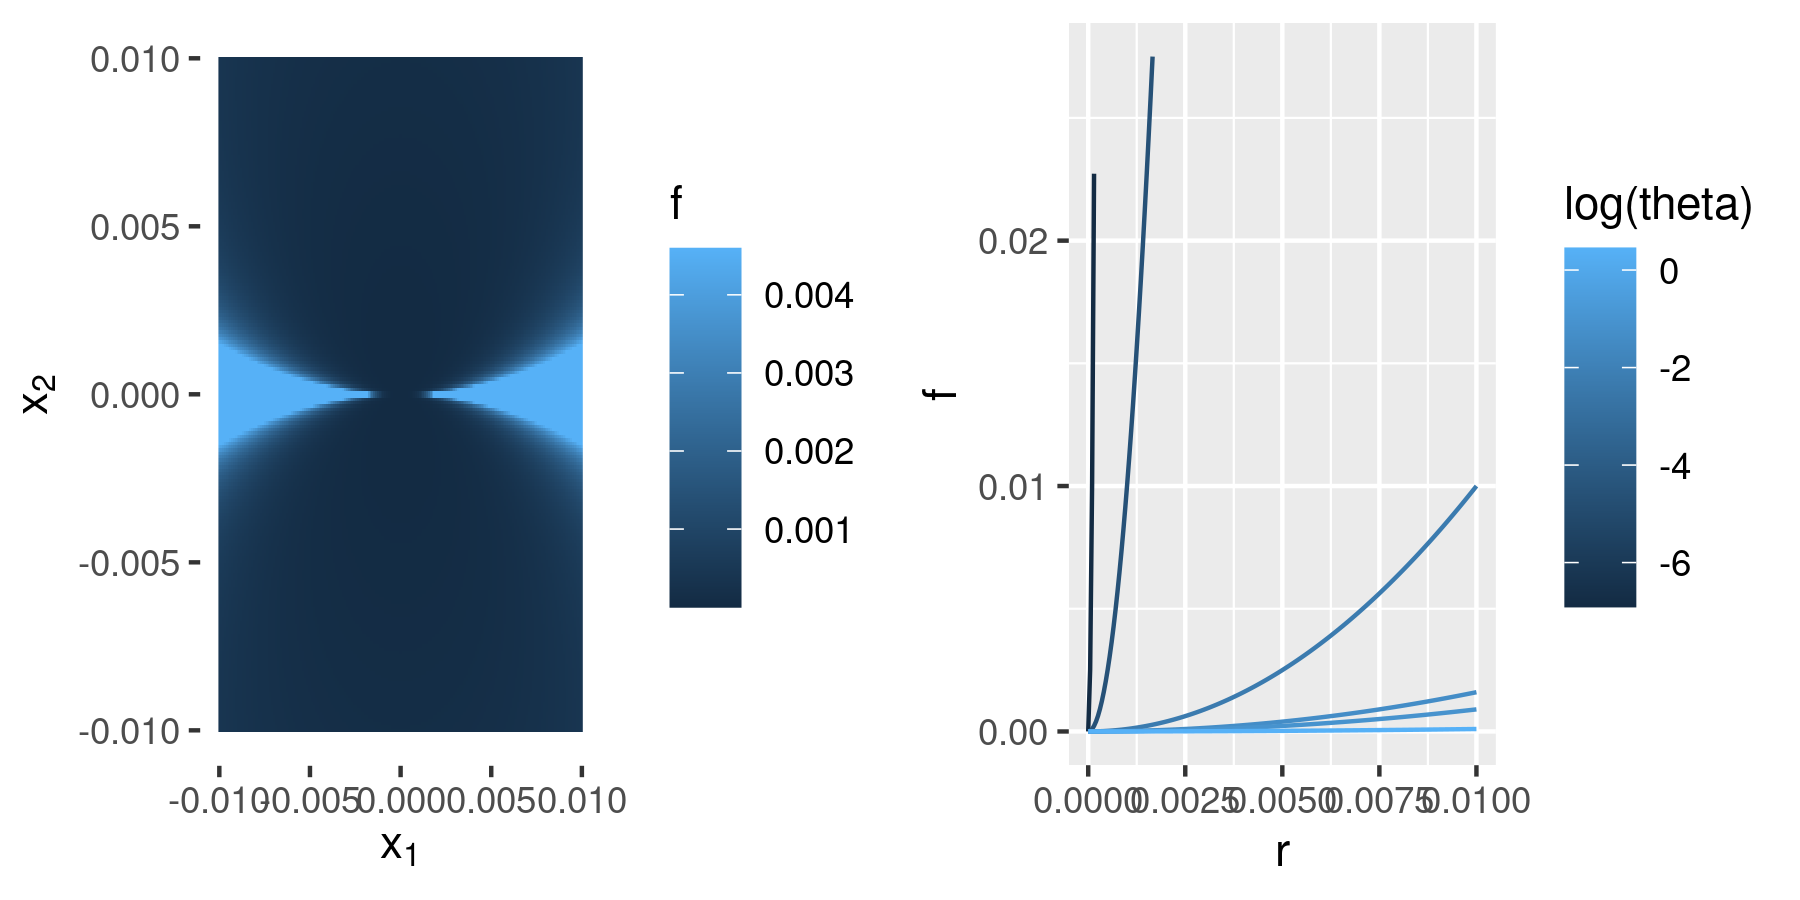
\includegraphics[width=0.980\linewidth,height=0.490\linewidth]{static_images/pathological_r2_example.png}
\caption{A plot of $f(x_1, x_2)$ from \exref{r2_pathological}.}
\figlabel{r2_pathological}
\centering
\end{figure}
%%%%%%%%%%%%%%%%%%%%%%%%%%%%%%%%%%%%%%%%%%%%%%%%%%%%%%%%%%%%%%%%%%%%%%%%%
%
\Figref{r2_pathological} contains a plot of $f(r, \theta)$, both over
$\mathbb{R}^2$ and along paths for particular choices of $\theta$.

We now show that $f$ has a directional derivative in every direction, but is not
Fr{\'e}chet differentiable.  By ordinary calculus, for any $\theta$,
$\fracat{\partial f(r, \theta)}{\partial r}{r=0} = 0$, so the directional
derivatives all exist and are identically $0$.  However, for any $r$, there
exists a $\theta(r)$ such that $r / |\sin(\theta(r))| = 1$.  For such a choice
of $\theta(r)$, the error in the linear approximation is $f(r, \theta(r)) - 0 =
1/2$, which does not go to zero as $r \rightarrow 0$.

\end{ex}
%%%%%%%%%%%%%%%%%%%%%%%%%%%%%%%%%%%%%%%%%%%%%%%%%%%%%%%%%%%%%%%%%%%%%%%%%

Fr{\'e}chet differentiability is only concerned with an infinitesimal
neighborhood.  The function can behave arbitrarily badly in a region just
outside the point at which the derivative is computed and retain Fr{\'e}che
differentiability. In this sense, Fr{\'e}chet differentiability is a desirable
but not sufficient requirement if we are interested in extrapolating using
linear approximations.  We illustrate this point in the

%%%%%%%%%%%%%%%%%%%%%%%%%%%%%%%%%%%%%%%%%%%%%%%%%%%%%%%%%%%%%%%%%%%%%%%%%
%%%%%%%%%%%%%%%%%%%%%%%%%%%%%%%%%%%%%%%%%%%%%%%%%%%%%%%%%%%%%%%%%%%%%%%%%
\begin{ex}\exlabel{r2_pathological_v2}
%
In \exref{r2_pathological} second derivative in a particular direction is given
by $\fracat{\partial^2 f(r, \theta)}{\partial r^2}{r=0} = \frac{1}{2 |\sin
\theta|}$, which can be made arbitrarily large by taking $\theta$ close to $0$
or to $\pi$.  We could modify $f(r, \theta)$ to be Fr{\'e}chet differentiable by
smoothly ``capping'' $1 / |\sin \theta|$ at some arbitrarily large value.
However, the ability to meaningfully extrapolate $f(r, \theta)$ in the direction
of a very large but finite second derivative will still be extremely limited.

In the context of \exref{r2_pathological}, fix some $0 < M < \infty$,
and define
%
\begin{align*}
%
\tilde{f}(r, \theta) := \begin{cases}
    f(r, \theta) & \textrm{when }\frac{1}{\abs{\sin(\theta)}} \le M \\
    0. & \textrm{when }\frac{1}{\abs{\sin(\theta)}} > M.
%
\end{cases}
%
\end{align*}
%
Then $\tilde{f}$ is continuous and Fr{\'e}chet differentiable at $r=0$. In this
case, for any $r$, $\sup_{\theta} r / |\sin(\theta(r))| = r / M$, so  both
$\lim_{r \rightarrow 0} \tilde{f}(r, \theta) \le \lim_{r \rightarrow 0} r^2 /
M^2 = 0$ and $\lim_{r \rightarrow 0} \tilde{f}(r, \theta) / r \le \lim_{r
\rightarrow 0}  r / M^2 = 0$.  (Note that $\tilde{f}$ is continuous only
at $r=0$, not on a ball centered at $0$.)

Despite being Fr{\'e}chet differentiable, the linear approximation may not
extrapolate well to any finite $r$.  In the direction $\theta = \sin^{-1}(1 /
M)$, the error of the linear extrapolation to any $r_0$ is still $\tilde{f}(r,
\theta) - 0 = M r_0^2$. Since Fr{\'e}chet differentiability requires only $M <
\infty$, the extraplation error can be arbitrarily large, even for Fr{\'e}chet
differentiable functions.

\end{ex}
%%%%%%%%%%%%%%%%%%%%%%%%%%%%%%%%%%%%%%%%%%%%%%%%%%%%%%%%%%%%%%%%%%%%%%%%%


\Exref{r2_pathological} is neither Fr{\'e}chet differentiable nor continuous,
whereas \exref{r2_pathological} is both Fr{\'e}chet differentiable and
continuous.  In general, however, Fr{\'e}chet differentiability is stronger than
continuity, in the sense that Fr{\'e}chet differentiability implies continuity,
but continuity does not imply Fr{\'e}chet differentiability \citep[Proposition
4.8 (d)]{zeidler:2013:functional}.  See also \citet[Example
1.9]{averbukh:1967:theory} for a simple example of a function on $\mathbb{R}^2$
that is continuous and directionally differentiable but not Fr{\'e}chet
differentiable.

The sort of pathology exhibited by \exref{r2_pathological, r2_pathological_v2}
requires some care to construct in $\mathbb{R}^2$, but requires some care to
avoid in infinite-dimensional spaces.  We now give an illustrative example in
the $\lp{p}$ spaces; since the result will be important for VB prior
sensitivity, we will state is as a lemma rather than merely an example.


%%%%%%%%%%%%%%%%%%%%%%%%%%%%%%%%%%%%%%%%%%%%%%%%%%%%%%%%%%%%%%%%%%%%%%%%%
%%%%%%%%%%%%%%%%%%%%%%%%%%%%%%%%%%%%%%%%%%%%%%%%%%%%%%%%%%%%%%%%%%%%%%%%%
\begin{ex}\exlabel{e_log_disocontinuous_v1}
%
Let $\q(\theta)$ and $\p(\theta)$ be densities relative to a continuous measure
$\lambda$.  Let $\gamma \in \lp{\p,p}$ with $1 \le p < \infty$, and define
%
\begin{align*}
%
f(\gamma) = \begin{cases}
\expect{\q(\theta)}{\log\left(1 + \gamma\right)}
    & \textrm{when }\inf_\theta \gamma(\theta) > -1 \\
-\infty & \textrm{otherwise}.
\end{cases}
%
\end{align*}
%
Then $f(\gamma)$ is trivially discontinuous at $\phiz$ since, for any $\gamma$
such that $\inf_\theta \gamma(\theta) = -\infty$,
%
\begin{align*}
%
f(\t \gamma) = -\infty \mathtxt{for any }\t > 0 \mathtxt{but} f(\phiz) = 0.
%
\end{align*}
%
\end{ex}
%%%%%%%%%%%%%%%%%%%%%%%%%%%%%%%%%%%%%%%%%%%%%%%%%%%%%%%%%%%%%%%%%%%%%%%%%

The problem with \exref{e_log_disocontinuous_v1} is not merely with
functions unbounded below, however.

%%%%%%%%%%%%%%%%%%%%%%%%%%%%%%%%%%%%%%%%%%%%%%%%%%%%%%%%%%%%%%%%%%%%%%%%%
%%%%%%%%%%%%%%%%%%%%%%%%%%%%%%%%%%%%%%%%%%%%%%%%%%%%%%%%%%%%%%%%%%%%%%%%%
\begin{ex}\exlabel{e_log_disocontinuous_v2}
%
In the setting of \exref{e_log_disocontinuous_v1}, assume further that, for any
$\epsilon \ge 0$, there exists a set $S_\epsilon$ such that $\p(S_\epsilon) \le
\epsilon$ and $\q(S_\epsilon) \ge \epsilon$.  Define
%
\begin{align*}
%
\tilde{f}(\gamma) = \begin{cases}
    f(\gamma) & \textrm{when }\inf_\theta \gamma(\theta) > -\infty \\
    0 & \textrm{otherwise}.
\end{cases}
%
\end{align*}
%
Now, with $\gamma$ such that $\inf_\theta \gamma(\theta) = -\infty$,
%
\begin{align*}
%
\tilde{f}(\t \gamma) = 0 \mathtxt{for any }\t > 0 \mathtxt{and} f(\phiz) = 0.
%
\end{align*}

However, $\tilde{f}$ is still discontinuous.  For any $\epsilon > 0$, let
$S_\epsilon$ be a set given in the assumption, and for $\delta > 0$, define
%
\begin{align*}
%
\gamma(\theta, \epsilon, \delta) :=
\begin{cases}
    %
    \delta - 1      & \textrm{ for }\theta\in S_\epsilon \\
    0      & \textrm{ for }\theta\notin S_\epsilon.
    %
\end{cases}
%
\end{align*}
%
Then $\gamma(\theta; \epsilon, \delta) \in \lp{\p,p}$ with.  Furthermore,
%
\begin{align*}
%
\norm{\gamma(\cdot;
\epsilon, \delta)}_{\p,p} =
    \left( \int_0^1 \phi(\theta)^p \p(\theta
)\lambda(d\theta)\right)^{1/p} \le{}& \epsilon^{1/p} (\delta - 1)  \mathand\\
%
\abs{\tilde{f}(\gamma(\cdot; \epsilon, \delta)) - \tilde{f}(\phiz)} =
    \expect{\q(\theta)}{\ind{\theta \in S_\epsilon}} \abs{\log(\delta)} \ge{}&
    \epsilon \abs{\log(\delta)}.
%
\end{align*}
%,
Take $\delta(\epsilon) = \exp(-\epsilon)$.  Then, for any sequence $\epsilon_n
\rightarrow 0$,
%
\begin{align*}
%
\abs{\tilde{f}(\phi(\cdot; \epsilon_n, \delta(\epsilon_n))) -
     \tilde{f}(\phiz)} \ge{} 1
\mathtxt{and}
\norm{\gamma(\cdot; \epsilon_n, \delta(\epsilon_n))}_p \rightarrow{} 0.
%
\end{align*}
%
So $\tilde{f}$ is discontinuous on an $\norm{\cdot}_p$ ball containing $\phiz$,
and cannot be Fr{\'e}chet differentiable.
%
\end{ex}
%%%%%%%%%%%%%%%%%%%%%%%%%%%%%%%%%%%%%%%%%%%%%%%%%%%%%%%%%%%%%%%%%%%%%%%%%




In \appref{proofs}, we state easy-to-verify (but technical) sufficient
conditions that allow us to establish \assuref{exchange_order}.  The key to
establishing \assuref{exchange_order} is the dominated convergence theorem
\citep[Theorem 16.8]{billingsley:1986:probability}, which states roughly that,
for some scalar-valued funciton $f(\theta, \tau)$,
%
\begin{align*}
%
\left. \frac{d}{d\tau} \int f(\theta, \tau) \mu(d\theta) \right|_{\tau=0} =
     \int \fracat{df(\theta, \tau)}{d\tau}{\tau=0}  \mu(d\theta)
%
\end{align*}
%
if there exists a dominating function $M(\theta) > 0$ such that
$\int M(\theta) \mu(d\theta) < \infty$ with $\abs{f(\theta, \tau)} < M(\theta)$
and $\abs{df(\theta, \tau) / d\tau} < M(\theta)$ in a neighborhood of $\tau=0$.



\hrulefill

NB: The problem with this proof is that it requires you to be able
to interchange integration and differentiation with $\q(\theta \vert \eta) \ind{A}$
for all sets $A$, which is not transparently a weaker assumption than
is required for the parametric.

%
It suffices to show that \assuref{exchange_order_q} implies
\assuref{exchange_order} for the perturbation given in \defref{prior_nl_pert}
when $\norminf{\phi} < \infty$.  Observe that $\log \ptil(\theta \vert \t) = \t
\phi(\theta)$, so
%
\begin{align*}
%
\expect{\q(\theta \vert \eta)}{\log \ptil(\theta \vert \t)} =
    \t \int \q(\theta \vert \eta) \phi(\theta) \mu(d\theta).
%
\end{align*}
%
Consider the derivative $\partial / \partial \eta$.  It suffices to show that
%
\begin{align*}
%
\MoveEqLeft
\norm{ \lim_{\eta \rightarrow \etaopt}
\int \phi(\theta)
    \left(\frac{\q(\theta \vert \eta) - \q(\theta \vert \etaopt)}
               {\eta - \etaopt} -
               \fracat{\partial \q(\theta \vert \eta)}{\partial \eta}{\etaopt}
           \right) \mu(d\theta) }_2
\\\le{}&
\norminf{\phi}
\lim_{\eta \rightarrow \etaopt}
\int
    \norm{\frac{\q(\theta \vert \eta) - \q(\theta \vert \etaopt)}
               {\eta - \etaopt} -
               \fracat{\partial \q(\theta \vert \eta)}{\partial \eta}{\etaopt}
           }_2  \mu(d\theta)
={} 0.
%
\end{align*}
%
The second derivative follows analogously.
%



\hrulefill


%%%%%%%%%%%%%%%%%%%%%%%%%%%%%%%%%%%%%%%%%%%%%%%%%%%%%%%%%%%%%%%%%%%%%%%%%%%%
%%%%%%%%%%%%%%%%%%%%%%%%%%%%%%%%%%%%%%%%%%%%%%%%%%%%%%%%%%%%%%%%%%%%%%%%%%%%
\todo{I think this is no longer necessary}
\begin{assu}\assulabel{dist_fun_nice}
%
% Let $\qtil(\theta \vert \eta)$ be a (integrable, but possibly unnormalized)
% density over the random variable $\theta$ parameterized by $\eta$ defined
% relative to a dominating measure $\mu$.
%
Assume that the map $\eta \mapsto \log \qtil(\theta \vert \eta)$ is twice
continuously differentiable. Let $\psi(\theta, \t)$ be a scalar-valued
$\mu$-measurable function of $\theta$ and $\t$.  Assume that the map $\t \mapsto
\psi(\theta, \t)$ is continuously differentiable.

Define the following shorthand notation:
%
\begin{align*}
%
\lqgrad{\theta \vert \eta} :={}&
    \fracat{\partial \log \qtil(\theta \vert \eta)}{\partial \eta}{\eta} \\
%
\lqhess{\theta \vert \eta} :={}&
    \fracat{\partial^2 \log \qtil(\theta \vert \eta)}
           {\partial \eta \partial \eta^T}{\eta} \\
%
\psigrad{\theta, \t} :={}& \fracat{\partial \psi(\theta, \t)}{\partial \t}{\t}.
%
\end{align*}
%
For a given $\t_0$ and $\eta_0$, assume there exists some neighborhood of
$\t_0$, $\ball_\t$, some neighborhood of $\eta_0$, $\ball_\eta$, and a
$\mu$-integrable $M_\psi(\theta)$ with $\int M_\psi(\theta) \mu(d\theta) <
\infty$ such that the following bounds hold for all $\eta, \t \in \ball_\eta
\times \ball_\t$:
%
\begin{enumerate}
%
\item \itemlabel{fundom}
$\qtil(\theta \vert \eta) \psi(\theta, \t) \le M_\psi(\theta)$.
%
\item \itemlabel{funqgraddom}
$\qtil(\theta \vert \eta) \norm{\lqgrad{\theta \vert \eta}}_2 \psi(\theta, \t) \le
M_\psi(\theta)$.
%
\item \itemlabel{funqhessdom}
$\qtil(\theta \vert \eta) \norm{\lqhess{\theta \vert \eta}}_2 \psi(\theta, \t) \le
M_\psi(\theta)$.
%
\item \itemlabel{fungradqgraddom}
$\qtil(\theta \vert \eta) \norm{\lqgrad{\theta \vert \eta}}_2 \psigrad{\theta, \t}
\le M_\psi(\theta)$.
%
\item \itemlabel{funqgradsqdom}
$\qtil(\theta \vert \eta) \norm{\lqgrad{\theta \vert \eta}}^2_2 \psi(\theta, \t) \le
M_\psi(\theta)$.
%
\end{enumerate}
%
\end{assu}
%%%%%%%%%%%%%%%%%%%%%%%%%%%%%%%%%%%%%%%%%%%%%%%%%%%%%%%%%%%%%%%%%%%%%%%%%%%%





%%%%%%%%%%%%%%%%%%%%%%%%%%%%%%%%%%%%%%%%%%%%%%%%%%%%%%%%%%%%%%%%%%%%%%%%%%%%%
%%%%%%%%%%%%%%%%%%%%%%%%%%%%%%%%%%%%%%%%%%%%%%%%%%%%%%%%%%%%%%%%%%%%%%%%%%%%%

\begin{proof}
%\prooflabel{pert_well_defined}
%\proofof{\thmref{pert_well_defined}}
%
First, consider the fact that perterubations are priors. It is clear that
$\mathscr{P}_{\mathrm{valid}} \subseteq \mathscr{P}_{\pbase,p}$, since one can
simply take $\t = 1$ for any $\palt \in \mathscr{P}_{\mathrm{valid}}$.  To show
that $\mathscr{P}_{\pbase,p} \subseteq \mathscr{P}_{\mathrm{valid}}$, it will
suffice to show that any element of $\mathscr{P}_{\pbase,p}$ is non-negative and
can be normalized.

Take $p \in [1, \infty)$ with $\phi \in \pertset$.  By definition, for $\phi \in
\pertset$, there exist $\beta > 0$, $\t \in [0,1]$, and $\palt(\theta)$ such
that
%
\begin{align*}
%
\pbase(\theta)^{1/p} + \frac{1}{p} \phi(\theta) ={}&
    \t \beta \palt(\theta)^{1/p} + (1- \t) \pbase(\theta)^{1/p}.
%
\end{align*}
%
From this it follows that $\ptil(\theta \vert \t \phi) \ge 0$, since $\t \in
[0,1]$.  Furthermore, for the same $\phi$,
%
\begin{align*}
%
\int \ptil(\theta \vert \phi) \mu(d\theta) ={}&
\int \left(\t \beta \palt(\theta)^{1/p} +
           (1- \t) \pbase(\theta)^{1/p} \right)^{p} \mu(d\theta)
\\\ge{}&
\t^p \beta^p \int \palt(\theta) \mu(d\theta) +
    (1- \t)^p \int \pbase(\theta) \mu(d\theta)
\\={}& \t^p \beta^p + (1- \t)^p > 0,
%
\end{align*}
%
and, by Jensen's inequality,
%
\begin{align*}
%
\int \ptil(\theta \vert \phi) \mu(d\theta) ={}&
2^p \int \left(\frac{1}{2} \t \beta \palt(\theta)^{1/p} +
           \frac{1}{2} (1- \t) \pbase(\theta)^{1/p} \right)^{p} \mu(d\theta)
\\\le{}&
%
2^{p-1} \left(
    \t^p \beta^p \int \palt(\theta) \mu(d\theta) +
    (1- \t)^p \int  \pbase(\theta)\mu(d\theta)
\right)
\\={}& 2^{p-1} \left( \t^p \beta^p + (1- \t)^p\right) < \infty.
%
\end{align*}

For $p = \infty$ and $\phi \in \pertset[\infty]$, it is clear that $\ptil(\theta
\vert \phi) = \pbase(\theta) \exp(\phi(\theta)) \ge 0$. As above, since $\phi
\in \pertset[\infty]$, there exist $\palt$, $\beta > 0$, and $\t \in [0,1]$ such
that
%
\begin{align*}
%
\phi(\theta) ={}&
    \t \log \palt(\theta) - (1-\t)\log \pbase(\theta) + \log \beta \Rightarrow\\
%
\int \ptil(\theta \vert \phi)\mu(d\theta) ={}&
    \beta \int \palt(\theta)^\t \pbase(\theta)^{1 - \t}\mu(d\theta)
\\={}&
\beta \int \pbase(\theta)
    \left( \frac{\palt(\theta)}{\pbase(\theta)}\right)^\t \mu(d\theta)
\\\le{}&
\beta \int \pbase(\theta)
    \frac{\palt(\theta)}{\pbase(\theta)}
    \ind{\palt(\theta) \ge \pbase(\theta)} \mu(d\theta) +
\\&
  \beta \int \pbase(\theta)
    \ind{\palt(\theta) < \pbase(\theta)} \mu(d\theta)
\\\le{}& 2\beta.
%
\end{align*}
%
This concludes the proof of PERT ARE PRIORS.

For PERTS VS BALL P, we show that, when $p \in [1, \infty)$ and
$\norm{\phi}_{\mu,p} < p$, then $\p(\theta \vert \phi)$ is normalizable. Um but
that is not necessary.  All we need to do is show that if $\phi \in \pertset$
then $\norm{\phi}_{\mu,p} < \infty$.

First, consider the case of general $\phi$ with $p \in [1, \infty)$. By Jensen's
inequality applied pointwise to the convex function $x \mapsto x^p$,
%
\begin{align*}
%
\abs{\pbase(\theta)^{1/p} + \frac{1}{p}\phi(\theta) }^{p} \le{}&
    \left(\pbase(\theta)^{1/p} + \frac{1}{p}\abs{\phi(\theta)} \right)^{p}
\\={}&
    2^p \left(\frac{1}{2}\pbase(\theta)^{1/p} +
              \frac{1}{2} \frac{1}{p}\abs{\phi(\theta)} \right)^{p}
\\\le{}&
    2^{p-1} \left(\pbase(\theta) + \frac{1}{p^p}\abs{\phi(\theta)}^p \right).
%
\end{align*}
%
Consequently,
%
\begin{align*}
%
\int \abs{\pbase(\theta)^{1/p} + \frac{1}{p}\phi(\theta) }^{p}
    \lambda(d\theta) \le{}&
2^{p-1} \int \left(\pbase(\theta) + \frac{1}{p}\abs{\phi(\theta)}^p \right)
    \lambda(d\theta)
\\={}&
    2^{p-1} \left(1 + \frac{1}{p^p}\norm{\phi}_p^p\right).
%
\end{align*}
%
So, as in \citep[Result 2]{gustafson:1996:local}, $\norm{\phi}_p < \infty$
implies that the prior can be normalized.

Continuing the case of general $\phi$ with $1 \le p < \infty$, by
convexity,\footnote{Apply the definition of convexity to the points $0$, $x$,
and $x + y$, and again to the points $0$, $y$, and $x+y$, then add the results.}
for any $x \ge y \ge 0$,
%
\begin{align*}
%
(x + y)^p \ge{} x^p + y^p \mathand
(x - y)^p \le{} x^p - y^p.
%
\end{align*}
%
Also note that, since $\pbase(\theta) \ge 0$,
%
\begin{align*}
%
\pbase(\theta)^{1/p} + \frac{1}{p}\phi(\theta) \le 0
\quad\Rightarrow\quad
\phi(\theta) \le 0 \mathand
\frac{1}{p} \abs{\phi(\theta)} - \pbase(\theta)^{1/p} \ge 0.
%
\end{align*}
%
We can thus write
%
\begin{align*}
%
\MoveEqLeft
\int \mathrm{sign}\left(\pbase(\theta)^{1/p} + \frac{1}{p}\phi(\theta)\right)
    \abs{\pbase(\theta)^{1/p} + \frac{1}{p}\abs{\phi(\theta)}}^{p} d\theta
\\={}&
    \int \left(\pbase(\theta)^{1/p} + \frac{1}{p}\phi(\theta)\right)^{p}
        \ind{\pbase(\theta)^{1/p} + \frac{1}{p}\phi(\theta) \ge 0}
        d\theta - \\&
    \int \left(\frac{1}{p}\abs{\phi(\theta)} - \pbase(\theta)^{1/p}\right)^{p}
        \ind{\pbase(\theta)^{1/p} + \frac{1}{p}\phi(\theta) < 0}
        d\theta
\\\ge{}&
    \int \left(\pbase(\theta) - \frac{1}{p^p}\abs{\phi(\theta)}^{p}\right)
        \ind{\pbase(\theta)^{1/p} + \frac{1}{p}\phi(\theta) \ge 0}
        d\theta - \\&
    \int \left(\frac{1}{p^p}\abs{\phi(\theta)}^p - \pbase(\theta)\right)
        \ind{\pbase(\theta)^{1/p} + \frac{1}{p}\phi(\theta) < 0}
        d\theta
\\={}&
    \int \pbase(\theta) d\theta - \frac{1}{p^p}\int \abs{\phi(\theta)}^p d\theta
\\={}&
    1 - \frac{1}{p^p} \norm{\phi}_p^p.
%
\end{align*}
%
The final line is non-negative when $\norm{\phi}_p \le p$.





Finally, consider $p = \infty$.  Since $\int \pbase(\theta) \lambda(d\theta) = 1$,
%
\begin{align*}
%
\exp(-\norminf{\phi}) \le{}
\abs{\int_0^1 \exp\left(\log \pbase(\theta) + \phi(\theta)\right) \lambda(d\theta)}
\le{}
\exp(\norminf{\phi}).
%
\end{align*}
%
so that $0 < \int \tilde{\p}(\theta \vert \phi) \lambda(d\theta) < \infty$
whenever $\norminf{\phi} < \infty$.  Furthermore,
%
\begin{align*}
%
\exp\left(\log \pbase(\theta) + \phi(\theta)\right) \ge 0.
%
\end{align*}
%
\end{proof}
%%%%%%%%%%%%%%%%%%%%%%%%%%%%%%%%%%%%%%%%%%%%%%%%%%%%%%%%%%%%%%%%%%%%%%%%%%%%%












\hrulefill







%
\begin{proof}[Proof of \lemref{logq_continuous}]\prooflabel{logq_continuous}
%
By \lemref{logq_derivs}, the mixed partial $ \eta, \t \mapsto \fracat{\partial^2
\expect{\q(\theta \vert \eta)} {\psi(\theta, \t)}}{\partial \eta \partial
\t}{\eta, \t}$ is a continuous combination of the terms
%
$\expect{\q(\theta \vert \eta)}
       {\lqgrad{\theta \vert \eta} \psigrad{\theta,\t}}$,
%
$\expect{\q(\theta \vert \eta)}
      {\lqgrad{\theta \vert \eta}}$, and
%
$\expect{\q(\theta \vert \eta)}
    {\psigrad{\theta,\t}}$.
%
By \assuref{exchange_order}, each of these expressions is continuous.  For
example,
%
\begin{align*}
%
\MoveEqLeft
\norm{\expect{\q(\theta \vert \eta)}
       {\lqgrad{\theta \vert \eta} \psigrad{\theta,\t}} -
   \expect{\q(\theta \vert \eta')}
          {\lqgrad{\theta \vert \eta'} \psigrad{\theta,\t'}}
      }_2 \\={}&
%
\norm{\int \left(
\q(\theta \vert \eta) \lqgrad{\theta \vert \eta} \psigrad{\theta,\t} -
\q(\theta \vert \eta') \lqgrad{\theta \vert \eta'} \psigrad{\theta,\t'}
\right)\mu(d\theta)
}_2  \le\\&
%
\int \norm{
\q(\theta \vert \eta) \lqgrad{\theta \vert \eta} \psigrad{\theta,\t} -
\q(\theta \vert \eta') \lqgrad{\theta \vert \eta'} \psigrad{\theta,\t'}
}_2 \mu(d\theta) \le\\&
%
\int \norm{
\left(\q(\theta \vert \eta) - \q(\theta \vert \eta')\right)
    \lqgrad{\theta \vert \eta} \psigrad{\theta, \t}
}_2 \mu(d\theta) + \\&\quad
%
\int \norm{
\q(\theta \vert \eta')
    \left( \lqgrad{\theta \vert \eta} - \lqgrad{\theta \vert \eta'} \right)
    \psigrad{\theta, \t}
}_2 \mu(d\theta) + \\&\quad
%
\int \norm{
\q(\theta \vert \eta')\lqgrad{\theta \vert \eta'}
    \left( \psigrad{\theta, \t} - \psigrad{\theta, \t'} \right)
}_2 \mu(d\theta).
%
\end{align*}
%
By ACTUALLY WE NEED THIS ASSUMPTION we can apply the dominated
convergence theorem to
each term in the final line of the preceding display, giving
%
\begin{align*}
%
\MoveEqLeft
\lim_{\eta' \rightarrow \eta} \lim_{\t' \rightarrow \t}
\norm{\expect{\q(\theta \vert \eta)}
       {\lqgrad{\theta \vert \eta} \psigrad{\theta,\t}} -
   \expect{\q(\theta \vert \eta')}
          {\lqgrad{\theta \vert \eta'} \psigrad{\theta,\t'}}
      }_2 \\\le{}&
%
\int \lim_{\eta' \rightarrow \eta} \lim_{\t' \rightarrow \t} \norm{
\left(\q(\theta \vert \eta) - \q(\theta \vert \eta')\right)
    \lqgrad{\theta \vert \eta} \psigrad{\theta, \t}
}_2 \mu(d\theta) + \\&\quad
%
\int \lim_{\eta' \rightarrow \eta} \lim_{\t' \rightarrow \t} \norm{
\q(\theta \vert \eta')
    \left( \lqgrad{\theta \vert \eta} - \lqgrad{\theta \vert \eta'} \right)
    \psigrad{\theta, \t}
}_2 \mu(d\theta) + \\&\quad
%
\int \lim_{\eta' \rightarrow \eta} \lim_{\t' \rightarrow \t} \norm{
\q(\theta \vert \eta')\lqgrad{\theta \vert \eta'}
    \left( \psigrad{\theta, \t} - \psigrad{\theta, \t'} \right)
}_2 \mu(d\theta) = 0,
%
\end{align*}
%
the final equality following from the continuity assumptions of
\assuref{dist_fun_nice}.

Similarly, $\fracat{\partial^2
\expect{\q(\theta \vert \eta)} {\psi(\theta, \t)}}{\partial \eta \partial
\eta^T}{\eta}$ involves terms of the form
%
\begin{align*}
%
\expect{\q(\theta \vert \eta)}
       {\lqgrad{\theta \vert \eta} \lqgrad{\theta \vert \eta}^T
        \psi(\theta,\t)}
       && \mathtxt{\assuitemref{dist_fun_nice}{funqgradsqdom}} \\
       %
\expect{\q(\theta \vert \eta)}
      {\lqgrad{\theta \vert \eta} \lqgrad{\theta \vert \eta}^T}
      && \mathtxt{\assuitemref{dist_fun_nice}{funqgradsqdom}} \\
%
\expect{\q(\theta \vert \eta)}
       {\lqhess{\theta \vert \eta}
        \psi(\theta,\t)}
       && \mathtxt{\assuitemref{dist_fun_nice}{funqhessdom}} \\
%
\expect{\q(\theta \vert \eta)}
       {\lqhess{\theta \vert \eta}},
       && \mathtxt{\assuitemref{dist_fun_nice}{funqhessdom}}
%
\end{align*}
%
to which we can apply \thmref{dct} by the corresponding assumption.  Reasoning
analogously to the other term, the conclusion follows.
%
\end{proof}
%
%%%%%%%%%%%%%%%%%%%%%%%%%%%%%%%%%%%%%%%%%%%%%%%%%%%%%%%%%%%%%%%%%%%%%%%%%%%%%
